\documentclass[11pt]{article} % article, report, or book

\usepackage[margin=1.0in]{geometry}
%\usepackage[parfill]{parskip}    		% Activate to begin paragraphs with an empty line rather than an indent
\usepackage{graphicx}				% Use pdf, png, jpg, or eps§ with pdflatex; use eps in DVI mode
\graphicspath{{../figures/}}
\usepackage{amsmath, bm}
\usepackage{color}
\usepackage[utf8]{inputenc} % allows for é
\usepackage{float} % allows for [H]
\usepackage{booktabs, caption, makecell}
\renewcommand\theadfont{\bfseries}
\usepackage{setspace}

%===================================================================
\title{A Discussion of Homoclinic Orbits in the Circular Restricted Three-Body Problem}
\author{Luke Bury \& Don Kuettel}
%===================================================================
\begin{document}
\maketitle
%===================================================================
\section{Introduction}
\color{red}\textbf{LUKE SECTION}\color{black}\\

\section{The Competition}
\color{red}\textbf{LUKE SECTION}\color{black}\\
%-------------------------------------------------------------------


%-------------------------------------------------------------------
\section{Circular Restricted Three Body Problem}
Before studying periodic orbits, their manifolds, and the process of locating homoclinic orbits, it is necessary to provide the reader a solid foundation of the Circular Restricted Three Body Problem (CR3BP) - the dynamical system in which the aforementioned trajectories are created and analyzed. In the CR3BP (Fig. \ref{f:CR3BP}), the origin of the system is set at the barycenter of the two main bodies in the system (e.g., the Earth \& Moon), and the frame rotates so these bodies remain stationary on the x-axis. The bodies are assumed to move in perfectly circular orbits and act as point masses from a gravitational perspective. The restricted problem is then to ascertain the motion of the third body whose mass is considered negligible. The system is typically normalized so that the masses of the two primary bodies sum to 1 (i.e., $m_1 = \mu$ and $m_2 = 1-\mu$, where $\mu = m_2/(m_1+m_2)$ is known as the three-body parameter), the distance between the primaries is 1, the orbital period period of the primaries is $2\pi$, and the gravitational constant G is equal to 1. Under these conditions, the equations of motion for the CR3BP are shown in Equations \ref{e:eomx}-\ref{e:eomz}:

\begin{align}
	\ddot{x} &= 2\dot{y} + x - (1-\mu)\left(\dfrac{x+\mu}{r_1^3}\right) - \mu\left(\dfrac{x-1+\mu}{r_2^3}\right) \label{e:eomx}\\
	\ddot{y} &= -2\dot{x} + y\left(-\dfrac{1-\mu}{r_1^3} - \dfrac{\mu}{r_2^3} + 1\right) \label{e:eomy}\\
	\ddot{z} &= z\left(-\dfrac{1 - \mu}{r_1^3} - \dfrac{\mu}{r_2^3}\right), \label{e:eomz}
\end{align} 

\noindent
where

\begin{align}
	r_1 & = \sqrt{\left(x + \mu\right)^2 + y^2 + z^2} \\
	r_2 & = \sqrt{\left(x - 1 + \mu\right)^2 + y^2 + z^2}.
\end{align}

\begin{figure}[H]
	\centering
	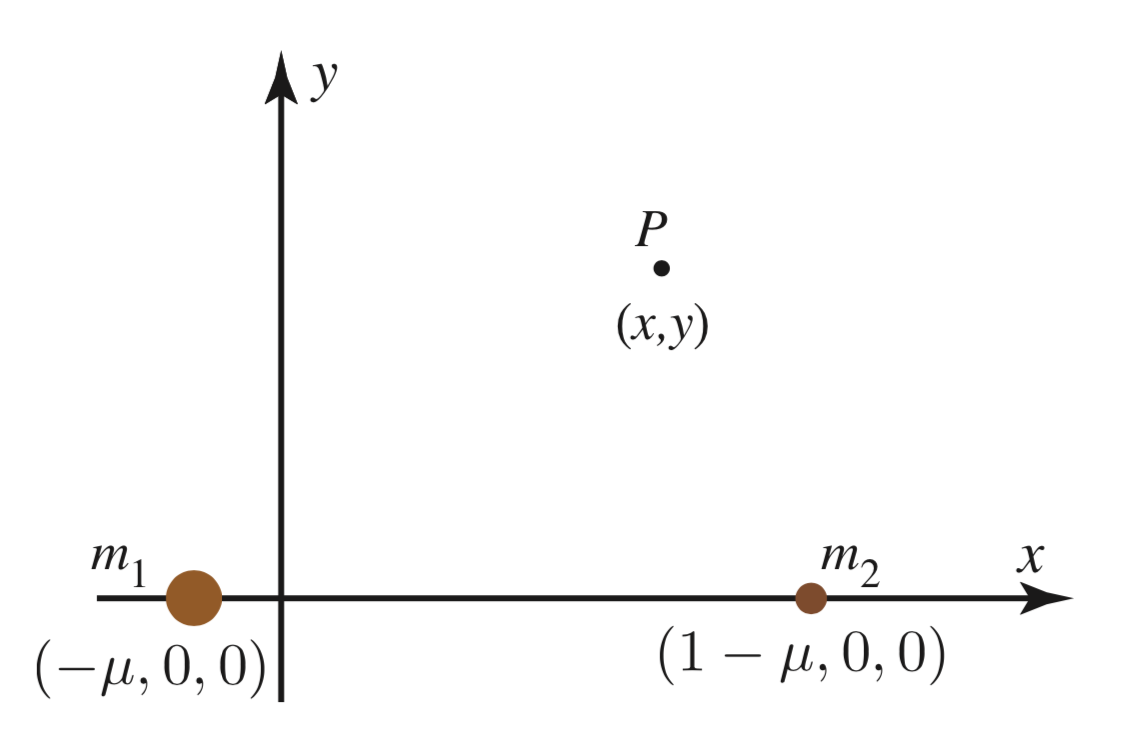
\includegraphics[width=4in]{CR3BP.png}\nonumber
	\caption{This figure shows the layout of the Circular Restricted Three-Body Problem \cite{KoonLoMarsdenRoss2011}}
	\label{f:CR3BP}
\end{figure}

In most simplified astrodynamic systems (e.g., Keplerian motion, CR3BP, $n$-body porblem, etc...), there are important parameters, known as integrals of motion, that are constant throughout the motion of a system that can be used to define the system. For example, the orbital elements of a trajectory in a Keplerian system are the system's integrals of motion. The integral of motion for the CR3PB is called the Jacobi constant and is given by 

\begin{equation}
	J = -\dot{x}^2-\dot{y}^2-\dot{z}^2+x^2+y^2 + \frac{2\left(1-\mu\right)}{r_1} + \frac{2\mu}{r_2}.
	\label{e:jacobi_constant}
\end{equation}

\noindent
For a given Jacobi constant, the motion of a particle is limited to certain regions of space due to the constraint that the velocity cannot have imaginary components. These restrictive regions, known as zero-velocity curves, are computed by setting the velocity in Equation \ref{e:jacobi_constant} to zero and mapping the resultant surfaces in the CR3PB. The motion of an object with a specific Jacobi constant in bound within its respective zero-velocity curve and can only cross the boundaries under some non-conservative force.

%-------------------------------------------------------------------
\subsection{Equilibrium Point Locations}
Complex dynamical system such as the CR3PB often times have equilibrium points that result in a constant solution to the system's differential equations. In the CR3BP, these points, known as Lagrange points, mark positions where the combined gravitational pull of the two large masses provides precisely the centripetal force required to orbit with them (i.e., the Lagrange points are stationary within the rotating system of the CR3BP). There are five such points labeled L$_1$ - L$_5$ located in the plane of the two primary masses. The first three Lagrange points lie on the line connecting the two primary bodies, and the last two points, L$_4$ and L$_5$, are located at the vertex of an equilateral triangle formed with the two primary bodies \cite{KoonLoMarsdenRoss2011}.

In order to find the location of the five equilibrium points in the CR3BP, the velocity and acceleration must be set to zero in the system's equations of motion. This results in the following equations:

\begin{align}
	0 & = x - (1-\mu)\left(\dfrac{x+\mu}{r_1^3}\right) - \mu\left(\dfrac{x-1+\mu}{r_2^3}\right) \label{e:eomx_zero}\\
	0 & = y\left(-\dfrac{1-\mu}{r_1^3} - \dfrac{\mu}{r_2^3} + 1\right) \label{e:eomy_zero}\\
	0 & = z. \label{e:eomz_zero}
\end{align}

\noindent
If $y$ is set to zero, a quintic equation in $x$ emerges. Solving this equation to first order results in the following location for the first three Lagrange points:

\begin{align}
	L_1 &= \left(1-\left(\frac{\mu}{3}\right)^{1/3},0,0\right)\label{e:L1_loc}\\
	L_2 &= \left(1+\left(\frac{\mu}{3}\right)^{1/3},0,0\right)\label{e:L2_loc}\\
	L_3 &= -\left(1+\left(\frac{5\mu}{12}\right),0,0\right). \label{e:L3_loc}
\end{align}

\noindent
Using Equations \ref{e:L1_loc}-\ref{e:L3_loc} as initial conditions, a Newton-Raphson iteration can then be used to numerically find the exact location of the first three Lagrange points to machine precision. Equations \ref{e:eomx_zero}-\ref{e:eomz_zero} can also be used to find the two triangular equilibrium points, L$_4$ and L$_5$. Since the equilibrium points form an equilateral triangle with the primary bodies, $r_1 = r_2 = 1$ is substituted into Equation \ref{e:eomx_zero} and Equation \ref{e:eomy_zero}. These equations are subsequently solved to provide the exact locations for the remaining equilibrium points:

\begin{align}
	L_4 &= \left(\frac{1}{2}-\mu, \frac{\sqrt{3}}{2},0\right)\\
	L_5 &= \left(\frac{1}{2}-\mu, -\frac{\sqrt{3}}{2},0\right).
\end{align}

\noindent
Using the Earth-Moon CR3BP three-body parameter ($\mu = 0.012155$), Table \ref{t:lagrange_points} shows the non-dimensional locations of the five Lagrange points to six significant digits. Additionally, Figure \ref{f:lagrange_points} graphically shows these locations along with a contour plot of the Earth-Moon CR3BP's zero-velocity curves for varying Jacobi constants. As Figure \ref{f:lagrange_points} shows, L$_1$, L$_2$, and L$_3$ lie at saddle points, while L$_4$ and L$_5$ lie at extrema values.

\begin{table}[! htbp]
	\centering 
	\caption{Summary of the Dimensionless Earth-Moon CR3BP Equilibrium Points}
	\begin{tabular}{cccc}
		\toprule\midrule
		\thead{Lagrange Point} & \thead{x} & \thead{y} & \thead{z} \\ 
	\midrule
		L$_1$ & 0.836893 & 0 & 0 \\
		L$_2$ & 1.15570 & 0 & 0 \\
		L$_3$ & -1.00506 & 0 & 0 \\
		L$_4$ & 0.487845 & 0.866025 & 0 \\
		L$_5$ & 0.487845 & -0.866025 & 0 \\
		\bottomrule
	\end{tabular}
	\label{t:lagrange_points}
\end{table}

\begin{figure}[H]
    \centering
    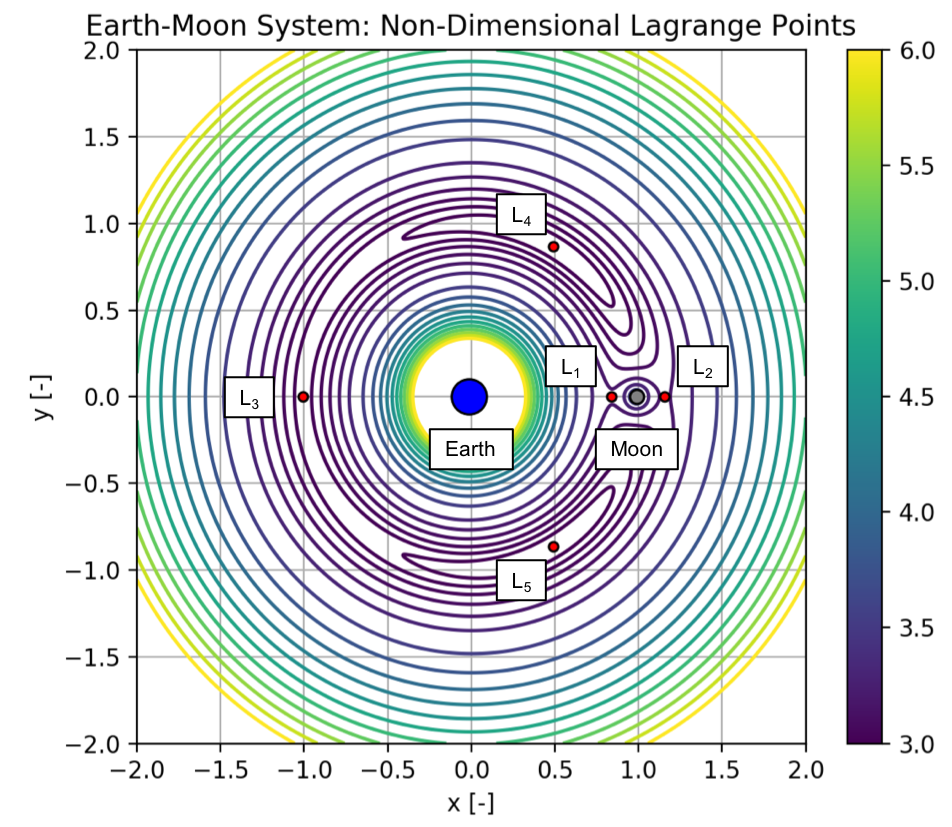
\includegraphics[width=6in]{zerovelocity_earthmoon.png}
    \caption{This figure depicts the the 5 equilibrium points and the zero-velocity curves in the non-dimensional Earth-Moon CR3BP system.}
    \label{f:lagrange_points}
\end{figure}

%-------------------------------------------------------------------

%-------------------------------------------------------------------
\subsection{Equilibrium Point Stability}
In this section a planar stability analysis is performed about each Lagrange point in the Earth-Moon CR3BP. This study entails linearizing the CR3BP equations of motion about each equilibrium solution and solving for the eigenvalues at the equilibrium point. The CR3BP equations of motion can be linearized by taking a Taylor series expansion of the ODE about each equilibrium point in the system. Neglecting higher order terms, the linearized equations of motion are give by

\begin{equation}
	\label{e:lin_eom}
	\delta\begin{bmatrix}\dot{x}\\\dot{y}\\\ddot{x}\\\ddot{y}\end{bmatrix} = Df\left(x^*,y^*,\dot{x}^*,\dot{y}^*\right)\begin{bmatrix}x\\y\\\dot{x}\\\dot{y}\end{bmatrix}
\end{equation}

\noindent
where,

\doublespacing
\begin{equation}
	\label{e:df_raw}
	Df\left(x,y,\dot{x},\dot{y}\right) = 
	\begin{bmatrix} 
		\frac{\partial \dot{x}}{\partial x} & \frac{\partial \dot{x}}{\partial y} & \frac{\partial \dot{x}}{\partial \dot{x}}  & \frac{\partial \dot{x}}{\partial \dot{y}} \\ 
		\frac{\partial \dot{y}}{\partial x} & \frac{\partial \dot{y}}{\partial y} & \frac{\partial \dot{y}}{\partial \dot{x}} & \frac{\partial \dot{y}}{\partial \dot{y}} \\
		\frac{\partial \ddot{x}}{\partial x} & \frac{\partial \ddot{x}}{\partial y} & \frac{\partial \ddot{x}}{\partial \dot{x}} & \frac{\partial \ddot{x}}{\partial \dot{y}} \\
		\frac{\partial \ddot{y}}{\partial x} & \frac{\partial \ddot{y}}{\partial y} & \frac{\partial \ddot{y}}{\partial \dot{x}} & \frac{\partial \ddot{y}}{\partial \dot{y}}
	\end{bmatrix}.
\end{equation}
\singlespacing

\noindent 
For the CR3BP, Equation \ref{e:df_raw} evaluates to 

\doublespacing
\begin{equation}
	\label{e:df_eval}
	Df\left(x,y,\dot{x},\dot{y}\right) = 
	\begin{bmatrix} 
		0 & 0 & 1  & 0 \\ 
		0 & 0 & 0 & 1 \\
		XX & XY & 0 & 2 \\
		YX & YY & -2 & 0
	\end{bmatrix}.
\end{equation}
\singlespacing

\noindent
where,

\begin{align}
	XX &= \frac{\mu - 1}{r_1^3} - \frac{\mu}{r_2^3} + \frac{3\mu\left(\mu+x-1\right)\left(\mu+x-1\right)}{r_2^5} - \frac{3\left(\mu+x\right)\left(\mu+x\right)\left(\mu-1\right)}{r_1^5} + 1 \\
	XY &= YX = \frac{3\mu y\left(\mu+x-1\right)}{r_2^5} - \frac{3y\left(\mu+x\right)\left(\mu-1\right)}{r_1^5} \\
	YY &= \frac{\mu - 1}{r_1^3} - \frac{\mu}{r_2^3} + \frac{3\mu y^2}{r_2^5} - \frac{3y^2\left(\mu-1\right)}{r_1^5} + 1
\end{align}

\noindent
By evaluating the matrix given in Equation \ref{e:df_eval} at the equilibrium points and finding the resulting eigenvalues of the matrix, the stability of that point can be studied.

\subsubsection{L$_1$, L$_2$, and L$_3$ Stability}
It was visually shown in Figure \ref{f:lagrange_points} that L$_1$, L$_2$, and L$_3$ were saddle points. By plugging in the locations of the equilibrium points given in Table \ref{t:lagrange_points} along with the Earth-Moon three-body parameter ($\mu = 0.012155$), this claim can be mathematically validated. 

\subsubsection*{L$_1$}
The evaluated $Df$ matrix for the L$_1$ Lagrange point is given by

\doublespacing
\begin{equation}
	\label{e:df_eval_L1}
	Df|_{L_1} = 
	\begin{bmatrix} 
		0 & 0 & 1  & 0 \\ 
		0 & 0 & 0 & 1 \\
		11.2955 & 0 & 0 & 2 \\
		0 & -4.1478 & -2 & 0
	\end{bmatrix}.
\end{equation}
\singlespacing

\noindent
where,

\begin{equation}
	\label{e:evals_L1}
	\lambda_{1,2} = \pm 2.9321 \text{ and } \lambda_{3,4} = \pm i2.3344.
\end{equation}

\noindent
As Equation \ref{e:evals_L1} shows, the L$_1$ equilibrium point has a positive, real eigenvalue that results in a dynamically unstable saddle point. Small departures from the equilibrium will grow exponentially with a time constant of $\tau = 1/real(\lambda_{3,4}) = 0.4284$. Re-dimensionalizing this value by the rotation rate of the Earth-Moon system ($\omega=2.665\times10^{-6}$ rad/sec) results in a time constant of $\tau\approx1.86$ days. In other words, a satellite parked at L$_1$ will wander off after a few days unless course corrections are made.

\subsubsection*{L$_2$}
The evaluated $Df$ matrix for the L$_2$ Lagrange point is given by

\doublespacing
\begin{equation}
	\label{e:df_eval_L2}
	Df|_{L_2} = 
	\begin{bmatrix} 
		0 & 0 & 1  & 0 \\ 
		0 & 0 & 0 & 1 \\
		7.3807 & 0 & 0 & 2 \\
		0 & -2.1903 & -2 & 0
	\end{bmatrix}.
\end{equation}
\singlespacing

\noindent
where,

\begin{equation}
	\label{e:evals_L2}
	\lambda_{1,2} = \pm 2.1586 \text{ and } \lambda_{3,4} = \pm i1.8626.
\end{equation}

\noindent
Similarly to the L$_1$ point, the L$_2$ Lagrange point has a positive, real eigenvalue that results in a dynamically unstable saddle point. The re-dimensionalized L$_2$ time constant is $\tau\approx2.33$ days. 

\subsubsection*{L$_3$}
The evaluated $Df$ matrix for the L$_3$ Lagrange point is given by

\doublespacing
\begin{equation}
	\label{e:df_eval_L3}
	Df|_{L_3} = 
	\begin{bmatrix} 
		0 & 0 & 1  & 0 \\ 
		0 & 0 & 0 & 1 \\
		3.0214 & 0 & 0 & 2 \\
		0 & -0.0107 & -2 & 0
	\end{bmatrix}.
\end{equation}
\singlespacing

\noindent
where,

\begin{equation}
	\label{e:evals_L3}
	\lambda_{1,2} = \pm 0.1779 \text{ and } \lambda_{3,4} = \pm i1.0104.
\end{equation}

\noindent
Once again, the evaluated $Df$ matrix has a positive, real eigenvalue resulting in the L$_3$ Lagrange point being unstable.The re-dimensionalized L$_3$ time constant is $\tau\approx4.30$ days.

\subsubsection{L$_4$ and L$_5$ Stability}
The stability analysis of the L$_4$ and L$_5$ Lagrange points yields a surprise. While these points correspond to local maxima of the total potential, they are stable due to a ``Coriolis'' force. Initially, a mass situated near L$_4$ or L$_5$ will tend to slide down the potential, but as it does, it picks up speed sending it into an orbit around the equilibrium point. To prove this, the evaluated $Df$ matrix for the L$_4$ and L$_5$ Lagrange points is given by

\doublespacing
\begin{equation}
	\label{e:df_eval_L45}
	Df|_{L_4,5} = 
	\begin{bmatrix} 
		0 & 0 & 1  & 0 \\ 
		0 & 0 & 0 & 1 \\
		0.7500 & \pm1.2675 & 0 & 2 \\
		\pm1.2675 & 2.2500 & -2 & 0
	\end{bmatrix}.
\end{equation}
\singlespacing

\noindent
where,

\begin{equation}
	\label{e:evals_L45}
	\lambda_{1,2} = \pm i0.9545 \text{ and } \lambda_{3,4} = \pm i0.2983.
\end{equation}

\noindent
As Equation \ref{e:evals_L45} shows, the L$_4$ and L$_5$ equilibrium points have purely imaginary eigenvalues in the Earth-Moon system resulting in Lyapunov stability. However, this is not always the case for a three body system. In order for the L$_4$ and L$_5$ Lagrange points to be stable, the primary masses of the system have to satisfy the follow inequality \cite{ScheersBook}

\begin{equation}
	\frac{m_1}{m_2} > \frac{25+\sqrt{621}}{2}\approx24.96.
\end{equation}

\noindent
For reference, $m_1/m_2=81.27$ for the Earth-Moon system.

%-------------------------------------------------------------------

%-------------------------------------------------------------------
\subsection{Periodic Orbits}

\subsubsection{Predictor-Corrector Method}

\subsubsection{Orbit Families}

%-------------------------------------------------------------------

%-------------------------------------------------------------------
\subsection{Periodic Orbit Manifolds}

%-------------------------------------------------------------------

%-------------------------------------------------------------------
\subsection{Poincar\'{e} Sections and Homoclinic Orbits}

%-------------------------------------------------------------------

%-------------------------------------------------------------------
\section{Conclusion}
\color{red}\textbf{LUKE SECTION}\color{black}\\

%===================================================================
\newpage
\bibliographystyle{plain}
\bibliography{../bibliography/appm5460.bib}

\end{document}  